\documentclass[hyperref={bookmarksopen=false}]{beamer} 

%\usepackage[english]{babel}
\usepackage[ngerman]{babel}
\usepackage{tikz}
%\usepackage[latin1]{inputenc}
\usepackage[utf8]{inputenc}
%fuer externe bilder
\usepackage{graphicx}
\usepackage{listings}
\usepackage{pgf}
\usepackage{tikz}
\usetikzlibrary{positioning,shadows,arrows}
\usetikzlibrary{automata,arrows}


\definecolor{tuRed}{cmyk}{0.1,1.0,0.8,0.0}

\useoutertheme[section]{tubs}

%\setbeamertemplate{itemize items}[ball]
%\setbeamertemplate{itemize items}[square]
\setbeamertemplate{itemize items}[tusquare]

\title[Teamprojekt im Lego-Labor]{TuringBrain IDE}
\subtitle{Ein Turing-Maschinen-Editor und -Simulator aus LEGO} 
\author[]{\tiny Vanessa Baier, Nils Breyer, Phillipp Neumann, Sven Schuster, David Wille}

\institute[TU Braunschweig, ITI]{Technische Universität Braunschweig, ITI}

\date{\today}

\instlogo{ips}
%\titlegraphic{iz}
\titlegraphic{title}

\begin{document}

\frame[plain]{\titlepage} 

\setbeamercolor{frametitle}{fg=white,bg=tu-red}
\frame{
        \frametitle{Inhalt}
        \tableofcontents
        }
\setbeamercolor{frametitle}{fg=black,bg=tu-grey}

\frame{
	\frametitle{Turingmaschine}
  		
}

\section{Hardware / Bauanleitung}

\frame{
	\frametitle{Turingmaschine}
        \begin{columns}
          \begin{column}{0.5\textwidth}
            \begin{center}
              \begin{tikzpicture}[->,shorten >=1pt,node
                distance=3cm,auto]
		% \draw[help lines] (0,-6) grid (12,6);
		\node[state] (q_0) {$q_c$};
              \end{tikzpicture}
            \end{center}

          \end{column}
          \begin{column}{0.5\textwidth}
            Zustand
          \end{column}
        \end{columns}


        \begin{columns}
          \begin{column}{0.5\textwidth}
            \begin{center}
              \begin{tikzpicture}[->,shorten >=1pt,node
                distance=3cm,auto]
		% \draw[help lines] (0,-6) grid (12,6);
                \node[state,initial] (q_f) {$q_F$};
              \end{tikzpicture}
              \quad
              \begin{tikzpicture}[->,shorten >=1pt,node
                distance=3cm,auto]
		% \draw[help lines] (0,-6) grid (12,6);
                \node[state,accepting] (q_f) {$q_F$};
              \end{tikzpicture}
            \end{center}
          \end{column}
          \begin{column}{0.5\textwidth}
                    Startzustand, Finalzustand
          \end{column}
        \end{columns}


        \begin{columns}
          \begin{column}{0.5\textwidth}
            	\begin{tikzpicture}[->,shorten >=1pt,node distance=3cm,auto]
		%\draw[help lines] (0,-6) grid (12,6);
		\node[state, initial] 	(q_0) {$q_0$}; 
		\node[state] (q_c) [right of = q_0] {$q_c$};
		\draw (q_0) to (q_c) node {$c / \#$};
              \end{tikzpicture}
          \end{column}
          \begin{column}{0.5\textwidth}
            Übergang
          \end{column}
        \end{columns}

  	\begin{center}

      \end{center}
}

\frame{
	\frametitle{Bedeutung der Bit Kombinationen}
  		\begin{figure}[!htb]
		\begin{center}
		\begin{tikzpicture}
		%\draw[help lines,scale=0.5] (0,0) grid (20,5);
		\draw[thick,scale=0.5] (1,1) rectangle +(1,1);
		\draw[thick,scale=0.5] (3,1) rectangle +(1,1);
		\draw[thick,scale=0.5,fill=tuRed] (1,3) rectangle +(1,1);
		\draw[thick,scale=0.5,fill=tuRed] (3,3) rectangle +(1,1);
		\draw (1.25,0.25) node[draw=none] {\#};

		\draw[thick,scale=0.5] (6,1) rectangle +(1,1);
		\draw[thick,scale=0.5,fill=tuRed] (8,1) rectangle +(1,1);
		\draw[thick,scale=0.5,fill=tuRed] (6,3) rectangle +(1,1);
		\draw[thick,scale=0.5] (8,3) rectangle +(1,1);
		\draw (3.75,0.25) node[draw=none] {0};

		\draw[thick,scale=0.5,fill=tuRed] (11,1) rectangle +(1,1);
		\draw[thick,scale=0.5] (13,1) rectangle +(1,1);
		\draw[thick,scale=0.5] (11,3) rectangle +(1,1);
		\draw[thick,scale=0.5,fill=tuRed] (13,3) rectangle +(1,1);
		\draw (6.25,0.25) node[draw=none] {1};

		\draw[thick,scale=0.5,fill=tuRed] (16,1) rectangle +(1,1);
		\draw[thick,scale=0.5,fill=tuRed] (18,1) rectangle +(1,1);
		\draw[thick,scale=0.5] (16,3) rectangle +(1,1);
		\draw[thick,scale=0.5] (18,3) rectangle +(1,1);
		\draw (8.75,0.25) node[draw=none] {2};
		\end{tikzpicture}
		\end{center}
		\end{figure}
}

\frame{
	\frametitle{Live Demo}
	TM erstellen + Sim  		
}

\frame{
	\frametitle{Features}
	Sim ohne Delay\\
	Export  		
}

\frame{
	\frametitle{Optional}
	Brainfuck\\
	2-Band-Sim (am Ende)\\
	Doku		
}

\frame{
	\frametitle{Brainfuck}
	\begin{figure}[!htb]
		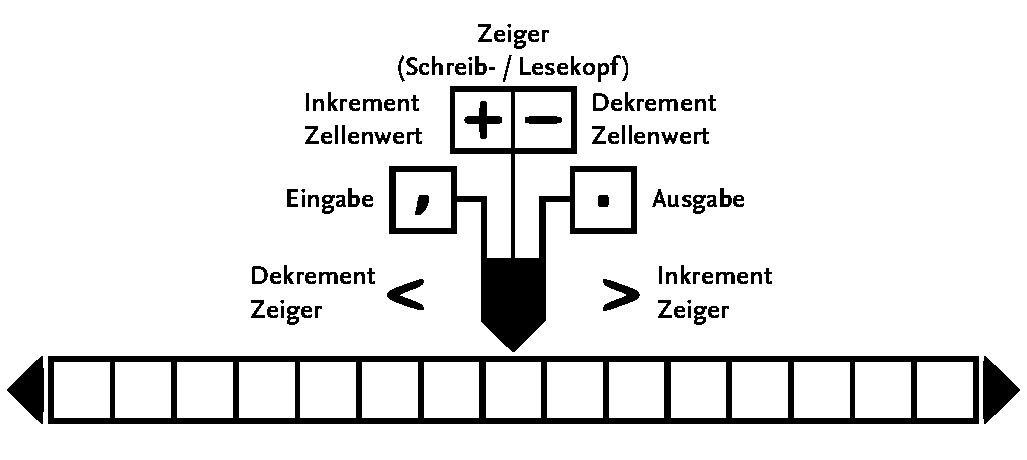
\includegraphics[scale=0.5]{graphics/brainfuck.pdf}
	\end{figure}
	
	Zusätzliche Befehle:
	\begin{itemize}
		\item $[$ - Wenn Zellenwert = \# : Springe zu zugehörigem $]$
		\item $]$ - Wenn Zellenwert $>$ \# : Springe zu zugehörigem $[$
	\end{itemize}
}

\frame{
  \begin{center}\huge
    Fragen?
  \end{center}

}

\end{document}   
